\begin{figure}[h]
\centering
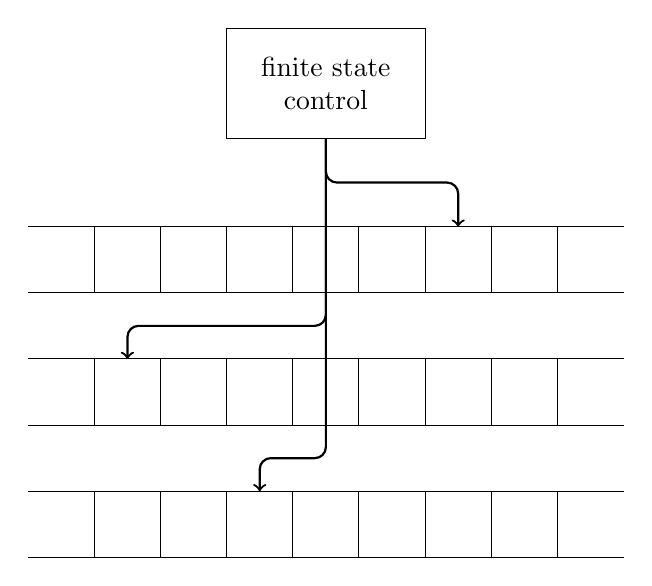
\begin{tikzpicture}[scale=1.4]
    \draw (5.5,1) rectangle (7.3,2);
    
    \node[text width = 2cm, align = center] at (6.4,1.5) {finite state control};

%Tape heads

    \draw[thick] [->] {[rounded corners] (6.4,1) -- (6.4,0.6) -- (7.6,0.6) -- (7.6,0.2)};

    \draw[thick] [->] {[rounded corners] (6.4,1) -- (6.4,-0.7) -- (4.6,-0.7) -- (4.6,-1)};

    \draw[thick] [->] {[rounded corners] (6.4,1) -- (6.4,-1.9) -- (5.8,-1.9) -- (5.8,-2.2)};

% First row of TM squares

	\draw (3.7,0.2) -- (4.3,0.2) -- (4.3,-0.4) -- (3.7,-0.4);
	\draw (4.3,0.2) rectangle (4.9,-0.4);
	\draw (4.9,0.2) rectangle (5.5,-0.4);
	\draw (5.5,0.2) rectangle (6.1,-0.4);
	\draw (6.1,0.2) rectangle (6.7,-0.4);
	\draw (6.7,0.2) rectangle (7.3,-0.4);
	\draw (7.3,0.2) rectangle (7.9,-0.4);
	\draw (7.9,0.2) rectangle (8.5,-0.4);
	\draw (9.1,-0.4) -- (8.5,-0.4) -- (8.5,0.2) -- (9.1,0.2);

%%Second row of TM squares
    \draw (3.7,-1) -- (4.3,-1) -- (4.3,-1.6) -- (3.7,-1.6);
	\draw (4.3,-1) rectangle (4.9,-1.6);
	\draw (4.9,-1) rectangle (5.5,-1.6);
	\draw (5.5,-1) rectangle (6.1,-1.6);
	\draw (6.1,-1) rectangle (6.7,-1.6);
	\draw (6.7,-1) rectangle (7.3,-1.6);
	\draw (7.3,-1) rectangle (7.9,-1.6);
	\draw (7.9,-1) rectangle (8.5,-1.6);
	\draw (9.1,-1.6) -- (8.5,-1.6) -- (8.5,-1) -- (9.1,-1);

%Third row of TM squares
    \draw (3.7,-2.2) -- (4.3,-2.2) -- (4.3,-2.8) -- (3.7,-2.8);
	\draw (4.3,-2.2) rectangle (4.9,-2.8);
	\draw (4.9,-2.2) rectangle (5.5,-2.8);
	\draw (5.5,-2.2) rectangle (6.1,-2.8);
	\draw (6.1,-2.2) rectangle (6.7,-2.8);
	\draw (6.7,-2.2) rectangle (7.3,-2.8);
	\draw (7.3,-2.2) rectangle (7.9,-2.8);
	\draw (7.9,-2.2) rectangle (8.5,-2.8);
	\draw (9.1,-2.8) -- (8.5,-2.8) -- (8.5,-2.2) -- (9.1,-2.2);    


\end{tikzpicture}


\caption{A $3$-tape DTM. The tape heads all move independently, but the DTM only works in one state at any time.}
\end{figure}